% Provenance (never printed): see sources/outline_sources.md (Year 3:
% Darcy's law; permeability; aquifer types; the groundwater-flow equation;
% pumping tests; solute transport, in principle).
% Brief: sources/book5/BRIEFS.md, ch. 23. Curves from figdata/bachelor-3/
% theis.py, flow_net.py and advection_dispersion.py; the site of Varden-3 from
% figdata/shared/region.py (read only). Exercise and problem values in the
% Book 5 scratch calculator calc/ch23.py. The wells, the dam, the tests and
% the solutes are invented.
\chapter{Hidrogeologi}\label{ch:b3:hydrogeology}

Sebuah sumur baru memompa \qty{2160}{m^3} air per hari dari batu gamping
yang terletak beberapa ratus meter di bawah sebuah peternakan. Mula-mula tidak ada
apa-apa yang terjadi pada sumur milik peternakan itu. Sebulan kemudian, muka airnya
hampir \qty{2}{m} lebih rendah, meskipun sumur itu berjarak satu kilometer dan stasiun pompa tidak pernah mengambil setetes pun darinya. Muka air di sekitar
sumur baru tidak turun merata: ia telah membentuk
kerucut, dan kerucut itu tumbuh dengan cepat melalui batuan tempat air
itu sendiri bergerak beberapa sentimeter per hari. Bab ini membangun fisika yang
meramalkan kedua besaran itu, yaitu penyebaran tekanan yang cepat dan
perjalanan air yang lambat, dari satu hukum empiris yang ditemukan pada 1856.
% ledger: heath:darcy

\begin{recall}
Porositas, permeabilitas, muka air tanah, air tanah, akuifer, mata air
dan sumur ada di buku-buku sekolah, beserta waktu tinggal air dan
air tanah fosil. Viskositas, hukum Poiseuille untuk aliran dalam tabung,
dan persamaan difusi ada di buku fisika. Fungsi galat
serta solusi persamaan difusi yang memakainya terdapat di
Bab~\ref{ch:b3:lithosphere-thermal-models}. Perbukitan Varden, wilayah fiktif seri ini,
dengan batu pasir, batu gamping, serpih, dan kapurnya,
adalah wilayah latihan sejak buku-buku sekolah.
\end{recall}

\section{Tinggi hidraulik dan hukum Darcy}\label{sec:b3:hydrogeology:darcy}

Air di bawah tanah bergerak dari tempat energi mekanik per satuan berat
tinggi ke tempat yang rendah. Karena geraknya lambat, energi kinetiknya
dapat diabaikan, dan energi tersebut memiliki dua bagian: tinggi air dan
tekanannya.

\begin{definition}[Tinggi hidraulik; gradien hidraulik]\label{def:b3:hydrogeology:head}
Yang disebut \emph{tinggi hidraulik}\index{tinggi hidraulik} di suatu titik pada
tanah jenuh adalah
\[
h = z + \frac{p}{\rho g} ,
\]
yaitu jumlah dari \emph{tinggi elevasi} $z$ titik itu di atas datum dan
\emph{tinggi tekanan} $p/(\rho g)$, dengan $p$ adalah tekanan air di atas
tekanan atmosfer. Ini adalah ketinggian yang dicapai air dalam sebuah
tabung, yakni piezometer yang hanya terbuka di titik itu. Yang disebut \emph{gradien
hidraulik}\index{gradien hidraulik} adalah $\nabla h$; besarnya antara dua
titik yang berjarak $L$ di sepanjang aliran ialah $\Delta h/L$.
\end{definition}

\begin{omfigure}
\centering
\begin{tikzpicture}[>=stealth, font=\small, x=1cm, y=1cm]
\fill[omLithAlluv!60] (0,-0.6) rectangle (7,3.2);
\fill[omSea!45] (0,-0.6) rectangle (7,1.9);
\draw[thick, brown!60!black] (0,3.2) -- (7,3.2);
\draw[omDef, dashed] (0,1.9) -- (7,1.9);
\node[omDef, font=\scriptsize, anchor=south east] at (6.9,1.92) {muka air tanah};
% piezometer
\fill[white] (3.3,0.4) rectangle (3.7,4.0);
\draw[thick] (3.3,0.7) -- (3.3,4.0); \draw[thick] (3.7,0.7) -- (3.7,4.0);
\draw[thick, densely dotted] (3.3,0.4) -- (3.3,0.7); \draw[thick, densely dotted] (3.7,0.4) -- (3.7,0.7);
\fill[omSea!70] (3.32,0.4) rectangle (3.68,2.6);
\draw[omDef, thick] (3.3,2.6) -- (3.7,2.6);
\fill (3.5,0.55) circle (0.06);
\node[font=\scriptsize, anchor=west] at (3.75,0.55) {saringan, di titik $P$};
% datum
\draw[black!60] (0,-0.6) -- (7,-0.6);
\node[font=\scriptsize, anchor=north west] at (0,-0.62) {datum, $z = 0$};
% heads, on the left of the tube
\draw[<->] (2.5,-0.6) -- node[left, font=\scriptsize] {$z$} (2.5,0.55);
\draw[<->] (2.5,0.55) -- node[left, font=\scriptsize] {$p/\rho g$} (2.5,2.6);
\draw[black!40, densely dashed] (2.4,0.55) -- (3.3,0.55);
\draw[black!40, densely dashed] (1.0,2.6) -- (3.3,2.6);
\draw[<->, thick, omThm] (1.1,-0.6) -- node[left, font=\scriptsize] {$h$} (1.1,2.6);
\node[font=\scriptsize, anchor=south] at (3.5,4.0) {piezometer};
\end{tikzpicture}

\par\smallskip{\small Piezometer, yakni tabung yang hanya terbuka pada saringannya. Air
di dalam tabung itu berada pada \omterm{def:b3:hydrogeology:head}{tinggi hidraulik} titik $P$, yaitu elevasi
$z$ ditambah tinggi tekanannya. Di sini, permukaan air dalam tabung berada di atas
muka air tanah, seperti pada tempat air naik menuju mata air atau
sungai.}\label{fig:b3:hydrogeology:head}
\end{omfigure}

Pada 1856 Henry Darcy, seorang insinyur Prancis, mengukur aliran air melalui
kolom pasir dan mendapati bahwa alirannya sebanding dengan kehilangan tinggi per satuan
panjang. Aliran ini laminar: air mengikuti garis alir yang terpisah.
% ledger: heath:darcy

\begin{theorem}[Hukum Darcy]\label{thm:b3:hydrogeology:darcy}
Dalam medium berpori yang jenuh, volume air yang melintasi satuan luas per
satuan waktu adalah
\[
\vec q = -K\,\nabla h ,
\]
dengan $K$ bergantung pada medium dan fluidanya. Pada medium yang porinya
berupa tabung lurus sejajar dengan jari-jari $a$ yang menempati fraksi $n$ dari
volume, hukum Poiseuille memberikan hukum ini dengan
\[
K = \frac{k\rho g}{\mu}, \qquad k = \frac{na^2}{8} ,
\]
dengan $\mu$ adalah viskositas air.
\end{theorem}
\index{hukum Darcy}

\begin{proof}
Pernyataan pertama adalah hukum empiris Darcy. Dalam tabung dengan jari-jari $a$
searah aliran, hukum Poiseuille memberikan kecepatan rata-rata $\bar u =
-(a^2/8\mu)\,\mathrm d(p + \rho gz)/\mathrm dl = -(a^2\rho g/8\mu)\,\mathrm
dh/\mathrm dl$, karena $p + \rho gz = \rho g h$. Tabung-tabung menempati
fraksi $n$ dari setiap penampang lintang, sehingga volume per satuan luas total adalah
$q = n\bar u = -(na^2/8)(\rho g/\mu)\,\mathrm dh/\mathrm dl$.
\end{proof}

Pori nyata tidak berbentuk tabung lurus; teorema ini menunjukkan bentuk hukum
dan bagaimana hukum itu berskala. Aliran berbanding lurus dengan gradien dan dengan kuadrat
ukuran pori, dan berbanding terbalik dengan viskositas: pasir yang sama
meloloskan air lebih cepat bila hangat.

\begin{definition}[Debit spesifik; konduktivitas hidraulik; permeabilitas intrinsik]\label{def:b3:hydrogeology:darcy}
Yang disebut \emph{debit spesifik}\index{debit spesifik} $\vec q$ adalah
volume air yang melintasi satuan luas medium, butiran dan pori
bersama-sama, per satuan waktu. Yang disebut \emph{konduktivitas
hidraulik}\index{konduktivitas hidraulik} $K$ adalah koefisien dalam \omterm{thm:b3:hydrogeology:darcy}{hukum
Darcy}, satuannya \unit{m/s} atau \unit{m/d}. Yang disebut \emph{permeabilitas
intrinsik}\index{permeabilitas intrinsik} medium adalah $k =
K\mu/(\rho g)$, dalam \unit{m^2}: nilainya hanya bergantung pada medium.
\end{definition}

\omterm{def:b3:hydrogeology:darcy}{Konduktivitas hidraulik} batuan membentang sepanjang dua belas orde
magnitudo, seperti sedikit besaran fisis lain. Dibaca dari grafik sebuah
survei klasik di bidang ini, rentang tipikal dalam meter per hari adalah: lempung
\num{e-7} sampai \num{e-4}; lanau dan loes \num{e-3} sampai 2; pasir lanauan 0.04 sampai
10; pasir bersih 0.3 sampai 150; kerikil 100 sampai 4000; serpih \num{e-8} sampai
\num{e-4}; batu pasir \num{e-5} sampai 0.4; batuan karbonat \num{e-4} bila
hanya retak, sampai beberapa ribu bila berongga; batuan beku dan batuan
metamorf di bawah \num{e-8} bila tidak retak, sampai beberapa bila
retak. Kebanyakan batuan juga mengalirkan air lebih baik sepanjang
perlapisannya daripada melintangnya.
% ledger: heath:darcy, heath:k-chart

\omterm{def:b3:hydrogeology:darcy}{Debit spesifik} adalah fluks melalui seluruh luas; air hanya mengalir
melalui pori, dan lebih cepat.

\begin{definition}[Kecepatan rembesan]\label{def:b3:hydrogeology:seepage}
Yang disebut \emph{kecepatan rembesan}\index{kecepatan rembesan} adalah $\vec v = \vec
q/n_e$, yaitu kecepatan rata-rata air di dalam pori, dengan $n_e$ sebagai
porositas efektif, yakni porositas pori-pori yang saling terhubung tempat air
mengalir.
\end{definition}

Pasir kasar dengan $K = \qty{60}{m/d}$, gradien 1 banding 1000, dan
porositas 0.20 membawa airnya dengan kecepatan \qty{0.3}{m/d}; lempung dengan $K =
\qty{e-4}{m/d}$, gradien 1 banding 10 dan porositas 0.50, pada
\qty{2e-5}{m/d}, kurang dari satu sentimeter per tahun. Air tanah tidak mengalir
di sungai bawah tanah, kecuali di gua-gua batu gamping dan tabung-tabung
lava. Ini semua hanya rata-rata: di tempat polutan bergerak, bagian
tercepatnya dapat bergerak beberapa kali lebih cepat.
% ledger: heath:velocity

\section{Akuifer}\label{sec:b3:hydrogeology:aquifers}

\begin{definition}[Akuifer tertekan dan akuifer bebas; akuitard]\label{def:b3:hydrogeology:aquifer-types}
Yang disebut \emph{akuifer bebas}\index{akuifer bebas} adalah akuifer yang
permukaan atasnya adalah muka air tanah. Yang disebut \emph{akuifer
tertekan}\index{akuifer tertekan} adalah akuifer yang ditutupi lapisan dengan
konduktivitas lebih rendah, sehingga air di dalamnya bertekanan: di sumur
yang mencapainya, air naik di atas puncak akuifer, sampai ke
permukaan potensiometrik. Lapisan dengan konduktivitas rendah yang memperlambat tetapi tidak
menghentikan aliran air antara akuifer adalah
\emph{akuitard}\index{akuitard}.
\end{definition}

\begin{definition}[Transmisivitas; storativitas; hasil spesifik]\label{def:b3:hydrogeology:storage}
Yang disebut \emph{transmisivitas}\index{transmisivitas} suatu akuifer dengan ketebalan
$b$ adalah $T = Kb$, yaitu debit per satuan lebar di bawah gradien satuan, dalam
\unit{m^2/d}. \emph{Storativitas}\index{storativitas} (atau
koefisien penyimpanan) $S$ adalah volume air yang dilepaskan per satuan luas
akuifer ketika \omterm{def:b3:hydrogeology:head}{tinggi hidraulik} turun sebesar satu satuan; besaran ini tak berdimensi.
Yang disebut \emph{hasil spesifik}\index{hasil spesifik} $S_y$ suatu batuan adalah volume
air yang mengalir keluar oleh gravitasi per satuan volume ketika muka
air tanah turun melaluinya.
\end{definition}

Kedua jenis akuifer melepaskan air dengan cara berbeda. Pada \omterm{def:b3:hydrogeology:aquifer-types}{akuifer tertekan}
\omterm{def:b3:hydrogeology:head}{tinggi hidraulik} turun tetapi pori tetap penuh: air memuai sedikit
dan akuifer, yang menanggung lebih banyak beban batuan di atasnya,
sedikit termampatkan. Pemuaian air saja melepaskan sekitar
\num{9e-7} meter kubik per meter kubik akuifer dan per meter \omterm{def:b3:hydrogeology:head}{tinggi hidraulik};
bersama dengan pemampatan, \omterm{def:b3:hydrogeology:storage}{storativitas} sebagian besar \omterm{def:b3:hydrogeology:aquifer-types}{akuifer tertekan} adalah
\num{e-5} sampai \num{e-3}. Pada \omterm{def:b3:hydrogeology:aquifer-types}{akuifer bebas} muka air tanah turun dan
pori di atasnya terkuras: \omterm{def:b3:hydrogeology:storage}{storativitasnya} adalah \omterm{def:b3:hydrogeology:storage}{hasil spesifik}, sekitar 0.1
sampai 0.3, seratus hingga sepuluh ribu kali lebih besar. \omterm{def:b3:hydrogeology:storage}{Transmisivitas}
akuifer yang dimanfaatkan berkisar dari kurang dari \qty{1}{m^2/d} di batuan retak
sampai \qty{100000}{m^2/d} di batu gamping berongga dan aliran lava. Bila
\omterm{def:b3:hydrogeology:head}{tinggi hidraulik} \omterm{def:b3:hydrogeology:aquifer-types}{akuifer tertekan} diturunkan dalam waktu lama, lempung di dalam dan
di sekitarnya terkuras dan memampat, dan tanah di atasnya amblas.
% ledger: heath:storage, heath:transmissivity

\begin{omfigure}
\centering
\begin{tikzpicture}[>=stealth, font=\small, x=1cm, y=1.1cm]
\begin{scope}
\clip (0,-1.3) -- (0,2.0) -- (3.5,2.9) -- (5,3.5) -- (7.5,4.2) -- (11,3.8) -- (11,-1.3) -- cycle;
\fill[lith sandstone] (0,-1.3) rectangle (11,4.5);
\fill[lith limestone] (0,1.8) -- (11,-0.95) -- (11,0.05) -- (0,2.8) -- cycle;
\fill[lith shale] (0,2.8) -- (11,0.05) -- (11,1.25) -- (0,4.0) -- cycle;
\fill[omLithLime!25] (0,4.0) -- (11,1.25) -- (11,4.5) -- (0,4.5) -- cycle;
\end{scope}
\draw[thick, brown!60!black] (0,2.0) -- (3.5,2.9) -- (5,3.5) -- (7.5,4.2) -- (11,3.8);
% water table in the chalk
\draw[omDef, dashed, thick] (4.5,3.0) .. controls (6,3.35) and (8.5,3.35) .. (11,2.8);
\node[omDef, font=\scriptsize, anchor=south] at (6.6,3.32) {muka air tanah};
% potentiometric surface of the limestone
\draw[omThm, densely dashdotted, thick] (1.4,2.36) -- (11,2.2);
\node[omThm, font=\scriptsize, anchor=south east, fill=white, inner sep=1pt] at (10.9,2.25) {permukaan potensiometrik batu gamping};
% well Varden-3
\draw[thick] (2.9,2.74) -- (2.9,1.05); \draw[thick] (3.1,2.8) -- (3.1,1.05);
\fill[omDef!35] (2.92,1.05) rectangle (3.08,2.33);
\draw[omThm, thick] (2.85,2.33) -- (3.15,2.33);
\node[font=\scriptsize, anchor=south] at (3.0,2.95) {Varden-3};
% labels
\node[font=\scriptsize, fill=white, inner sep=1pt] at (7.5,0.45) {batu gamping: akuifer tertekan};
\node[font=\scriptsize, fill=white, inner sep=1pt] at (7.5,1.5) {serpih: lapisan penyekat};
\node[font=\scriptsize, fill=white, inner sep=1pt] at (8.4,2.8) {kapur: akuifer bebas};
\node[font=\scriptsize, fill=white, inner sep=1pt] at (7.5,-0.8) {batu pasir};
\node[font=\scriptsize, fill=white, inner sep=1pt, align=center] at (0.8,1.75) {batu gamping\\singkapan};
\draw[->, omDef, thick] (0.8,3.0) -- (0.8,2.3);
\node[omDef, font=\scriptsize, anchor=south] at (0.8,3.0) {imbuhan};
\end{tikzpicture}

\par\smallskip{\small Penampang skematis lapisan penutup Perbukitan Varden
dari barat ke timur, tidak dalam skala. Kapur menampung \omterm{def:b3:hydrogeology:aquifer-types}{akuifer bebas}
di bawah muka air tanahnya. Batu gamping Jura mendapat pengisian ulang di tempat ia
tersingkap dan tertekan di bawah serpih: di sumur Varden-3 pada
soal, dibor menembus serpih dan hanya terbuka pada batu gamping, air
naik hingga permukaan potensiometrik, jauh di atas puncak
akuifer tetapi di bawah permukaan tanah.}\label{fig:b3:hydrogeology:aquifers}
\end{omfigure}
% ledger: region:name

\section{Persamaan aliran air tanah}\label{sec:b3:hydrogeology:flow-equation}

\begin{theorem}[Persamaan aliran air tanah]\label{thm:b3:hydrogeology:flow-equation}
Pada \omterm{def:b3:hydrogeology:aquifer-types}{akuifer tertekan} dengan \omterm{def:b3:hydrogeology:storage}{transmisivitas} $T$ dan \omterm{def:b3:hydrogeology:storage}{storativitas} $S$ yang konstan,
dengan aliran horizontal, tinggi $h(x, y, t)$ memenuhi
\[
S\,\frac{\partial h}{\partial t} = T\nabla^2h + W ,
\]
$W$ adalah volume air yang ditambahkan per satuan luas dan waktu oleh pengisian ulang atau
diambil oleh pemompaan (bernilai negatif). Pada aliran tunak tanpa sumber, $\nabla^2h =
0$.
\end{theorem}
\index{persamaan aliran air tanah}

\begin{proof}
Tinjau sebuah kolom akuifer dengan luas $\mathrm dx\,\mathrm dy$. Aliran per
satuan lebar melalui seluruh ketebalannya adalah $-T\nabla h$, dari \omterm{thm:b3:hydrogeology:darcy}{hukum Darcy}
dikali $b$. Aliran masuk bersih adalah $-\nabla\cdot(-T\nabla h)\,\mathrm dx\,\mathrm
dy = T\nabla^2h\,\mathrm dx\,\mathrm dy$. Air yang tersimpan dalam kolom
berubah dengan laju $S\,(\partial h/\partial t)\,\mathrm dx\,\mathrm dy$,
sesuai definisi $S$. Kekekalan massa, dengan massa jenis air dianggap
konstan dalam neraca, menyamakan tampungan dengan aliran masuk ditambah sumber.
\end{proof}

Ini adalah persamaan difusi dari buku fisika, dengan difusivitas hidraulik
$T/S$ menggantikan difusivitas termal. Untuk batu gamping tertekan dengan
$T = \qty{450}{m^2/d}$ dan $S = \num{2e-4}$, difusivitasnya adalah
\qty{2.25e6}{m^2/d}: perubahan tinggi menyebar sejauh \qty{1}{km} dalam
sekitar $L^2S/T$, setengah hari. Batu gamping yang sama, tak tertekan, dengan $S =
0.2$, membutuhkan waktu seribu kali lebih lama. Tekanan menyebar cepat, air
bergerak lambat: kedua angka dari pembukaan tadi.

\begin{proposition}[Aliran radial tunak ke sumur]\label{prop:b3:hydrogeology:thiem}
Sebuah sumur memompa $Q$ dari \omterm{def:b3:hydrogeology:aquifer-types}{akuifer tertekan} dengan \omterm{def:b3:hydrogeology:storage}{transmisivitas} $T$, alirannya
tunak dan radial. Antara dua jarak $r_1 < r_2$ dari sumur, penurunannya
berbeda sebesar
\[
s_1 - s_2 = \frac{Q}{2\pi T}\ln\frac{r_2}{r_1} .
\]
\end{proposition}

\begin{proof}
Melalui setiap lingkaran berjari-jari $r$ di sekeliling sumur, aliran masuknya adalah $Q = 2\pi r
T\,\mathrm dh/\mathrm dr$. Mengintegralkan $\mathrm dh = (Q/2\pi T)\,\mathrm
dr/r$ dari $r_1$ ke $r_2$, dan menuliskan $s = h_0 - h$, diperoleh hasilnya.
\end{proof}

Pada dua dimensi, aliran tunak digambarkan dengan \omterm{def:b3:hydrogeology:flow-net}{jaring aliran}.

\begin{definition}[Jaring aliran]\label{def:b3:hydrogeology:flow-net}
Yang disebut \emph{jaring aliran}\index{jaring aliran} adalah gambar aliran air tanah tunak dalam
penampang homogen dan isotropik yang dibentuk oleh dua keluarga kurva: ekuipotensial,
yaitu garis dengan tinggi yang sama, dan garis alir yang diikuti air. Garis
alir memotong ekuipotensial tegak lurus, dan dalam jaring aliran
jaraknya diatur sedemikian rupa sehingga selnya berbentuk persegi lengkung.
\end{definition}

\begin{method}[Rembesan dari jaring aliran]\label{met:b3:hydrogeology:flow-net}
\leavevmode
\begin{enumerate}
\item Gambarkan batasnya: batas kedap air adalah garis alir; badan air
  dasarnya, tempat tinggi tetap, adalah ekuipotensial.
\item Gambarkan $N_d$ penurunan tinggi di antara tinggi tertinggi dan terendah, $\Delta h
  = H/N_d$, dan garis alir yang membentuk $N_f$ saluran aliran, dengan coba-coba,
  hingga setiap sel berbentuk persegi lengkung.
\item Setiap saluran membawa $K\Delta h$ per satuan panjang tegak lurus
  penampang, panjang dan lebar persegi saling menghapuskan: totalnya adalah $q =
  KHN_f/N_d$.
\end{enumerate}
\end{method}

\begin{omfigure}
\centering
\begin{tikzpicture}
\begin{axis}[width=0.95\linewidth, height=0.36\linewidth, axis equal image,
  xmin=-60, xmax=60, ymin=-20, ymax=13, xlabel={$x$ (\unit{m})}, ylabel={$z$ (\unit{m})},
  tick label style={font=\scriptsize}, label style={font=\small}, clip=false]
% computed in figdata/bachelor-3/flow_net.py
\fill[omLithAlluv!35] (axis cs:-60,-20) rectangle (axis cs:60,0);
\fill[omSea!40] (axis cs:-60,0) rectangle (axis cs:-10,11.2);
\fill[omSea!40] (axis cs:10,0) rectangle (axis cs:60,1.2);
\fill[black!35] (axis cs:-10,0) -- (axis cs:-10,12.5) -- (axis cs:-5,12.5) -- (axis cs:10,0) -- cycle;
\pgfplotsinvokeforeach{1,...,9}{
  \addplot[omThm, thin, unbounded coords=jump] table[x=x, y=z] {figdata/out/bachelor-3-flow_net-h-#1.dat};}
\pgfplotsinvokeforeach{1,...,4}{
  \addplot[omMeth, thick, unbounded coords=jump] table[x=x, y=z] {figdata/out/bachelor-3-flow_net-psi-#1.dat};}
\draw[very thick] (axis cs:-60,-20) -- (axis cs:60,-20);
\node[font=\scriptsize, anchor=south] at (axis cs:45,-19.6) {batuan kedap air};
\node[font=\scriptsize, align=center] at (axis cs:-36,6) {waduk, \qty{10}{m} di atas\\air hilir};
\node[font=\scriptsize, anchor=south] at (axis cs:35,1.4) {air hilir};
\node[font=\scriptsize] at (axis cs:-4,4) {bendungan};
\end{axis}
\end{tikzpicture}

\par\smallskip{\small Rembesan di bawah bendungan selebar \qty{20}{m} pada lapisan
pasir setebal \qty{20}{m}, waduk \qty{10}{m} di atas air
hilir, dihitung dengan menyelesaikan persamaan Laplace untuk tinggi dan untuk
fungsi arus. Garis tipis: ekuipotensial, satu setiap satu meter tinggi.
Garis tebal: empat garis alir yang, bersama dasar bendungan dan lantai,
membatasi lima saluran aliran. Rembesan yang dihitung adalah $0.51\,KH$ per meter
bendungan; \omterm{def:b3:hydrogeology:flow-net}{jaring aliran} memberikan $KH \times 5/10 = 0.50\,KH$.}\label{fig:b3:hydrogeology:flow-net}
\end{omfigure}

\section{Uji pemompaan}\label{sec:b3:hydrogeology:pumping}

Aliran tunak menuju sumur jarang terjadi: keadaan tunak yang baru mungkin butuh berbulan-bulan atau
bertahun-tahun, atau tidak pernah tercapai. Pada 1935 Theis, dari Survei Geologi
AS, memberikan penurunan muka air di sekitar sumur yang dipompa pada laju konstan sebagai
fungsi waktu, dari situ uji beberapa jam atau hari menghasilkan
\omterm{def:b3:hydrogeology:storage}{transmisivitas} dan \omterm{def:b3:hydrogeology:storage}{storativitas} akuifer.
% ledger: heath:theis

\begin{theorem}[Solusi Theis]\label{thm:b3:hydrogeology:theis}
Sumur yang menembus penuh \omterm{def:b3:hydrogeology:aquifer-types}{akuifer tertekan} tak terhingga dan homogen,
dengan \omterm{def:b3:hydrogeology:storage}{transmisivitas} $T$ dan \omterm{def:b3:hydrogeology:storage}{storativitas} $S$ mulai dipompa pada $t = 0$ dengan
laju konstan $Q$. Penurunan muka air pada jarak $r$ adalah
\[
s(r, t) = \frac{Q}{4\pi T}\,W(u), \qquad u = \frac{r^2S}{4Tt}, \qquad
W(u) = \int_u^\infty\frac{\mathrm e^{-y}}{y}\,\mathrm dy = -\gamma - \ln u +
u - \frac{u^2}{2\cdot2!} + \frac{u^3}{3\cdot3!} - \cdots,
\]
dengan $\gamma = \num{0.5772}$. $W$ disebut fungsi sumur.
\end{theorem}
\index{Solusi Theis}

\begin{proof}
Dalam bentuk radial, persamaan alirannya adalah $S\,\partial s/\partial t =
T\,r^{-1}\partial_r(r\,\partial_rs)$, dengan $s = 0$ pada $t = 0$, $s \to 0$ ketika
$r \to \infty$ dan $2\pi rT\,\partial_rs \to -Q$ ketika $r \to 0$. Tidak ada
besaran yang memuat panjang atau waktu secara tersendiri, maka coba $s = f(u)$ dengan $u =
r^2S/4Tt$. Karena $\partial_ru = 2u/r$ dan $\partial_tu = -u/t$, $r\,\partial_rs =
2uf'$, $r^{-1}\partial_r(r\,\partial_rs) = (4u/r^2)(uf')'$ dan $\partial_ts =
-(u/t)f'$. Dengan mengalikan persamaan dengan $r^2/(4Tu)$ diperoleh $(uf')' = -uf'$:
dengan $g = uf'$, $g' = -g$, dan $g = c\,\mathrm e^{-u}$. Syarat sumur, $2\pi T\cdot2uf' \to -Q$ ketika $u \to 0$, memberikan $c =
-Q/4\pi T$, dan $f(\infty) = 0$ memberikan $f(u) = (Q/4\pi T)\int_u^\infty
\mathrm e^{-y}y^{-1}\,\mathrm dy$. Deret diperoleh dari
$W(u) = -\gamma - \ln u + \int_0^u(1 - \mathrm e^{-y})\,y^{-1}\,\mathrm dy$,
konstantanya adalah konstanta Euler, dengan mengintegralkan suku demi suku.
\end{proof}

\begin{proposition}[Pendekatan Cooper--Jacob]\label{prop:b3:hydrogeology:cooper-jacob}
Jika $u \le 0.05$, penurunan muka air Theis mendekati
\[
s = \frac{2.3\,Q}{4\pi T}\log_{10}\frac{2.25\,Tt}{r^2S} :
\]
Jika diplot terhadap $\log_{10}t$, penurunan muka air berupa garis lurus yang kenaikannya per
siklus logaritma, $\Delta s$, memberikan $T = 2.3\,Q/(4\pi\Delta s)$, dan
perpotongannya dengan $s = 0$, pada $t_0$, memberikan $S = 2.25\,Tt_0/r^2$.
\end{proposition}
\index{Pendekatan Cooper--Jacob}

\begin{proof}
Untuk $u$ kecil, deret menjadi $W \approx -\gamma - \ln u = \ln(\mathrm
e^{-\gamma}/u) = \ln(0.5615\cdot4Tt/r^2S) = \ln(2.25\,Tt/r^2S)$; suku
berikutnya, $u$, paling besar \num{0.05}, kurang dari \qty{2}{\percent} dari $W$ di sana.
Karena $\ln x = 2.3\log_{10}x$, penurunan muka air naik $2.3\,Q/4\pi T$ setiap
kenaikan waktu sepuluh kali, dan menjadi nol ketika $2.25\,Tt_0 = r^2S$.
\end{proof}

\begin{omfigure}
\begin{tikzpicture}
\begin{groupplot}[group style={group size=2 by 1, horizontal sep=1.5cm},
  width=0.48\linewidth, height=0.4\linewidth,
  tick label style={font=\scriptsize}, label style={font=\small}, title style={font=\small}]
\nextgroupplot[xmode=log, xlabel={$1/u$}, ylabel={$W(u)$}, xmin=0.1, xmax=1e4, ymin=0, ymax=9,
  title={fungsi sumur},
  legend style={font=\scriptsize, at={(0.03,0.97)}, anchor=north west}]
% computed in figdata/bachelor-3/theis.py
\addplot[omDef, thick] table[x=invu, y=W] {figdata/out/bachelor-3-theis-wu.dat};
\addlegendentry{Theis $W(u)$}
\addplot[omThm, densely dashed, thick] table[x=invu, y=Wcj] {figdata/out/bachelor-3-theis-cj.dat};
\addlegendentry{$-\gamma - \ln u$}
\addplot[black!40, densely dotted, forget plot] coordinates {(20,0) (20,9)};
\node[font=\scriptsize, black!60, anchor=west] at (axis cs:24,0.6) {$u = 0.05$};
\nextgroupplot[xmode=log, xlabel={waktu sejak pemompaan dimulai (\unit{min})}, ylabel={penurunan muka air (\unit{m})},
  xmin=0.5, xmax=5000, ymin=0, ymax=3.4, title={Varden-3, $r = \qty{60}{m}$},
  legend style={font=\scriptsize, at={(0.03,0.97)}, anchor=north west}]
\addplot[only marks, mark=*, mark size=1.3pt] table[x=tmin, y=s] {figdata/out/bachelor-3-theis-test.dat};
\addlegendentry{terukur}
\addplot[omMeth, thick, domain=0.973:5000, samples=2] {0.87221*log10(x/0.973132)};
\addlegendentry{Garis Cooper--Jacob}
\addplot[black!40, densely dotted, forget plot] coordinates {(11.5,0) (11.5,3.4)};
\end{groupplot}
\end{tikzpicture}

\par\smallskip{\small Kiri, fungsi sumur Theis terhadap $1/u$ pada
sumbu logaritmik, dan pendekatan garis lurusnya: keduanya menyatu ketika $u <
0.05$ (titik-titik). Kanan, penurunan muka air yang tercatat di sumur pengamatan
uji Varden-3 pada soal, \qty{60}{m} dari sumur yang dipompa, dan
garis lurus yang dicocokkan dengan titik-titik setelah \qty{11.5}{min}, saat $u <
0.05$: kemiringannya memberikan $T$, perpotongannya $S$.}\label{fig:b3:hydrogeology:theis}
\end{omfigure}
% ledger: heath:theis, heath:jacob

\begin{definition}[Kerucut depresi]\label{def:b3:hydrogeology:cone}
Yang disebut \emph{kerucut depresi}\index{kerucut depresi} sumur yang dipompa adalah
depresi muka air tanah, atau permukaan potensiometrik,
di sekeliling sumur; gradiennya makin curam ke arah sumur, tempat semua air harus lewat.
yang harus dilalui air.
\end{definition}

Karena penurunan muka air mematuhi persamaan linear, kerucut beberapa sumur
dapat dijumlahkan. Pada \omterm{def:b3:hydrogeology:aquifer-types}{akuifer tertekan}, dengan \omterm{def:b3:hydrogeology:storage}{storativitasnya} yang kecil, kerucut tumbuh cepat
dan kerucut sumur-sumur tetangga segera saling bertumpang tindih; pada \omterm{def:b3:hydrogeology:aquifer-types}{akuifer bebas},
yang harus menguras pori-porinya, kerucut tumbuh lambat. Kerucut berhenti
tumbuh hanya bila ia sudah menangkap cukup imbuhan, atau mengurangi cukup
debit alami akuifer ke sungai dan mata air, untuk mencapai keseimbangan
dengan pemompaan. Penarikan air besar dari \omterm{def:b3:hydrogeology:aquifer-types}{akuifer tertekan} menjangkau jauh: pada 1981
sekitar \qty{277000}{m^3/d} yang dipompa dari akuifer Kapur di dataran
pesisir Atlantik, di Virginia dan Carolina Utara, telah membentuk
kerucut yang saling bertumpang tindih di seluruh wilayah itu.
% ledger: heath:cone

\begin{omfigure}
\begin{tikzpicture}
\begin{groupplot}[group style={group size=2 by 1, horizontal sep=1.5cm},
  width=0.48\linewidth, height=0.4\linewidth, y dir=reverse,
  tick label style={font=\scriptsize}, label style={font=\small}, title style={font=\small}]
\nextgroupplot[xlabel={jarak dari sumur (\unit{m})}, ylabel={penurunan muka air (\unit{m})},
  xmin=0, xmax=3000, ymin=0, ymax=6, title={kerucut satu sumur},
  scaled x ticks=false, xticklabel style={/pgf/number format/1000 sep={}},
  legend style={font=\scriptsize, at={(0.97,0.03)}, anchor=south east}]
% computed in figdata/bachelor-3/theis.py
\addplot[omThm!50, thick] table[x=r, y=s] {figdata/out/bachelor-3-theis-cone-1.dat};
\addlegendentry{1 hari}
\addplot[omThm!80, thick] table[x=r, y=s] {figdata/out/bachelor-3-theis-cone-10.dat};
\addlegendentry{10 hari}
\addplot[omThm!60!black, thick] table[x=r, y=s] {figdata/out/bachelor-3-theis-cone-100.dat};
\addlegendentry{100 hari}
\nextgroupplot[xlabel={$x$ (\unit{m})}, ylabel={penurunan muka air (\unit{m})},
  xmin=-1500, xmax=1900, ymin=0, ymax=9, title={dua sumur, 10 hari},
  scaled x ticks=false, xticklabel style={/pgf/number format/1000 sep={}},
  legend columns=3, legend style={font=\scriptsize, at={(0.5,0.985)}, anchor=north,
  /tikz/every even column/.append style={column sep=3pt}}]
\addplot[omDef, densely dashed] table[x=x, y=s1] {figdata/out/bachelor-3-theis-interf.dat};
\addlegendentry{sumur di 0}
\addplot[omMeth, densely dashed] table[x=x, y=s2] {figdata/out/bachelor-3-theis-interf.dat};
\addlegendentry{sumur di 400 m}
\addplot[black, thick] table[x=x, y=stot] {figdata/out/bachelor-3-theis-interf.dat};
\addlegendentry{keduanya}
\end{groupplot}
\end{tikzpicture}

\par\smallskip{\small Kerucut Theis dari sumur Varden-3 ($Q =
\qty{2160}{m^3/d}$, $T = \qty{450}{m^2/d}$, $S = \num{2e-4}$), penurunan muka air
digambar ke bawah. Kiri, setelah 1, 10, dan 100 hari: kerucut makin dalam sebesar
jumlah yang sama untuk setiap kelipatan sepuluh kali waktu dan melebar tanpa batas pada
akuifer tak hingga. Kanan, dua sumur serupa berjarak \qty{400}{m} setelah 10 hari: penurunan muka air
saling menjumlah, \qty{5.5}{m} di tengah keduanya, bukan \qty{2.7}{m}
untuk satu sumur.}\label{fig:b3:hydrogeology:cone}
\end{omfigure}
% ledger: heath:cone, heath:storage

\begin{inthefield}[Uji pemompaan]
\begin{minipage}[t]{0.55\linewidth}\vspace{0pt}
Sebelum uji pemompaan, ahli hidrogeologi mencatat muka air dalam
sumur selama beberapa waktu, untuk mengetahui tren yang akan menjadi latar uji ini
di atasnya. Pompa kemudian bekerja pada laju tetap, dijaga stabil dan diukur oleh
meter pada pipa buang, selama beberapa jam hingga beberapa hari. Pada setiap
sumur pengamatan, sedikitnya tiga buah pada jarak berbeda bila
memungkinkan, kedalaman muka air di bawah titik ukur tetap dibaca pada
waktu yang diketahui dengan tepat, banyak di menit-menit awal dan lebih sedikit kemudian: dengan
pita baja berskala, atau pita listrik yang elektrodanya menutup sirkuit
saat menyentuh air. Kini, transduser tekanan terendam yang digantung di
sumur, dihubungkan ke perekam elektronik, mencatat muka air hampir
terus-menerus.
\end{minipage}\hfill
\begin{minipage}[t]{0.42\linewidth}\vspace{0pt}
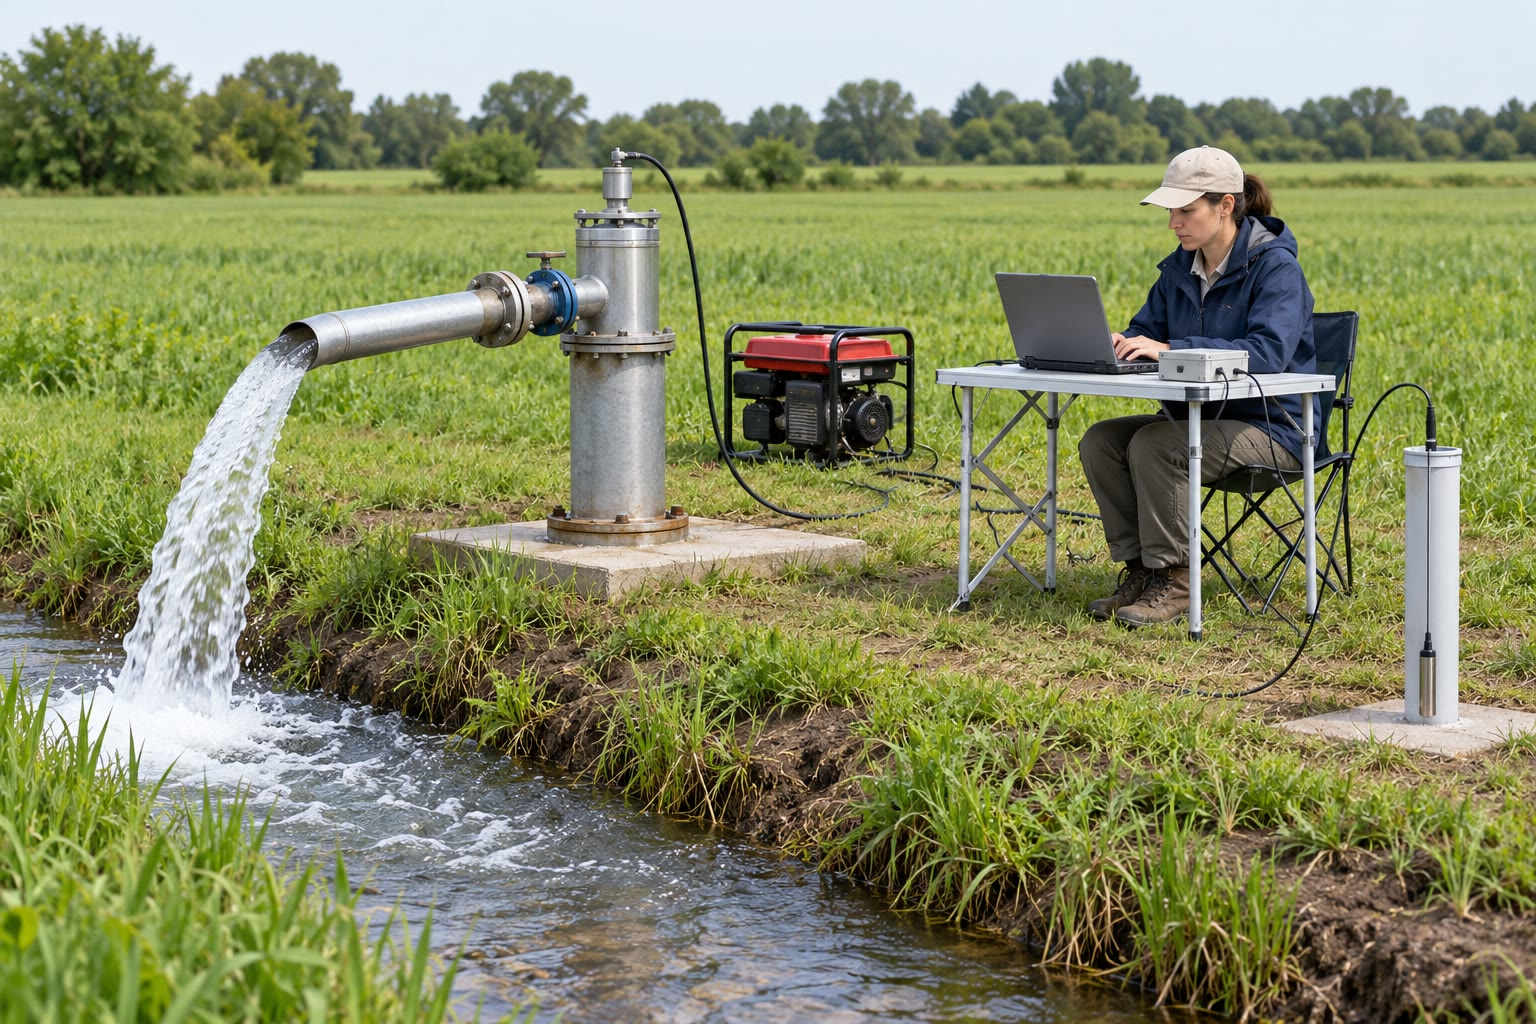
\includegraphics[width=\linewidth]{images/book5/ai/b3-pumping-test.jpg}

{\scriptsize Uji pemompaan: pipa buang sumur yang dipompa, generator, dan
ahli hidrogeologi yang mencatat muka air sumur pengamatan
di laptop (ilustrasi buatan AI).}
\end{minipage}
\end{inthefield}
% ledger: heath:theis, heath:jacob, heath:water-levels, usgs:transducers

\section{Transpor zat terlarut}\label{sec:b3:hydrogeology:transport}

Zat terlarut dalam air tanah terbawa bersama air, dengan
\omterm{def:b3:hydrogeology:seepage}{kecepatan rembesan}, dan menyebar selama perjalanannya: air di pori-pori tetangga
bergerak dengan laju dan lintasan yang berbeda, dan zat terlarut
juga berdifusi.

\begin{definition}[Dispersi hidrodinamik; dispersivitas]\label{def:b3:hydrogeology:ade}
\emph{Dispersi hidrodinamik}\index{dispersi hidrodinamik} adalah
penyebaran zat terlarut dalam air tanah yang mengalir akibat variasi
kecepatan air dari pori ke pori dan oleh difusi molekular. Sepanjang
arah aliran, dispersi itu dinyatakan dengan koefisien dispersi $D = \alpha_Lv + D^*$,
dengan $v$ \omterm{def:b3:hydrogeology:seepage}{kecepatan rembesan}, $D^*$ difusivitas molekular efektif, dan
$\alpha_L$, suatu panjang, ialah
\emph{dispersivitas}\index{dispersivitas} longitudinal medium.
\end{definition}

\begin{theorem}[Persamaan adveksi--dispersi]\label{thm:b3:hydrogeology:ade}
Sepanjang aliran satu dimensi dengan \omterm{def:b3:hydrogeology:seepage}{kecepatan rembesan} $v$ tetap,
konsentrasi $C(x, t)$ zat terlarut yang tidak bereaksi memenuhi
\[
\frac{\partial C}{\partial t} = D\,\frac{\partial^2C}{\partial x^2} -
v\,\frac{\partial C}{\partial x} .
\]
Jika konsentrasi dijaga pada $C_0$ di $x = 0$ mulai dari $t = 0$, dalam medium
yang mula-mula bebas zat terlarut,
\[
\frac{C}{C_0} = \frac12\left[\operatorname{erfc}\frac{x - vt}{2\sqrt{Dt}} +
\mathrm e^{vx/D}\operatorname{erfc}\frac{x + vt}{2\sqrt{Dt}}\right] .
\]
\end{theorem}
\index{persamaan adveksi--dispersi}

\begin{proof}
Dalam sebuah irisan berpenampang satuan dan panjang $\mathrm dx$, dengan
porositas efektif $n_e$, zat terlarut yang tersimpan adalah $n_eC\,\mathrm dx$. Fluksnya
$n_e(vC - D\,\partial C/\partial x)$, terbawa bersama air dan tersebar oleh
dispersi seperti hukum Fick menyebarkan zat yang berdifusi. Kekekalan massa memberikan
$n_e\partial_tC = -\partial_x[n_e(vC - D\partial_xC)]$, itulah persamaannya. Bahwa
rumus itu memenuhinya dan syarat-syaratnya diterima di sini;
\cref{exo:b3:hydrogeology:12} memeriksa penyebarannya.
\end{proof}

Dalam kerangka yang bergerak bersama air, $\xi = x - vt$, persamaan itu menjadi
persamaan difusi, dan front menyebar sebagai $\sqrt{2Dt} = \sqrt{2\alpha_L
vt} = \sqrt{2\alpha_Lx}$: lebar front bertumbuh sebagai akar kuadrat
dari jarak yang ditempuh.

\begin{definition}[Faktor retardasi]\label{def:b3:hydrogeology:retardation}
Zat terlarut yang teradsorpsi pada butir, dalam kesetimbangan dan sebanding
dengan konsentrasinya, bergerak lebih lambat daripada air. Nilai
\emph{faktor retardasi}\index{faktor retardasi (sorpsi)} adalah
\[
R = 1 + \frac{\rho_bK_d}{n} ,
\]
$\rho_b$ menyatakan massa jenis curah kering medium, $n$ porositasnya dan
$K_d$ koefisien distribusi, yaitu massa yang teradsorpsi per satuan massa
padatan dibagi konsentrasi dalam air. Zat terlarut bergerak dengan laju $v/R$
dan tersebar dengan $D/R$.
\end{definition}

\begin{omfigure}
\begin{tikzpicture}
\begin{groupplot}[group style={group size=2 by 1, horizontal sep=1.5cm},
  width=0.48\linewidth, height=0.4\linewidth,
  tick label style={font=\scriptsize}, label style={font=\small}, title style={font=\small}]
\nextgroupplot[xlabel={waktu (hari)}, ylabel={$C/C_0$ pada \qty{100}{m}},
  xmin=0, xmax=1000, ymin=0, ymax=1.05, title={kurva tembus},
  legend style={font=\scriptsize, at={(0.97,0.03)}, anchor=south east}]
% computed in figdata/bachelor-3/advection_dispersion.py
\addplot[omDef, thick] table[x=t, y=c1] {figdata/out/bachelor-3-advection_dispersion-btc.dat};
\addlegendentry{$\alpha_L = \qty{1}{m}$}
\addplot[omMeth, thick] table[x=t, y=c3] {figdata/out/bachelor-3-advection_dispersion-btc.dat};
\addlegendentry{$\alpha_L = \qty{3}{m}$}
\addplot[omThm, thick] table[x=t, y=c10] {figdata/out/bachelor-3-advection_dispersion-btc.dat};
\addlegendentry{$\alpha_L = \qty{10}{m}$}
\addplot[black, thick, densely dashed, forget plot] table[x=t, y=cR] {figdata/out/bachelor-3-advection_dispersion-btc.dat};
\node[font=\scriptsize, anchor=west, align=left] at (axis cs:640,0.45) {$\alpha_L = \qty{3}{m}$,\\ $R = 3$};
\addplot[black!40, densely dotted, forget plot] coordinates {(200,0) (200,1.05)};
\nextgroupplot[xlabel={jarak (\unit{m})}, ylabel={$C/C_0$ setelah 150 hari},
  xmin=0, xmax=160, ymin=0, ymax=1.05, title={profil},
  legend style={font=\scriptsize, at={(0.03,0.03)}, anchor=south west}]
\addplot[omDef, thick] table[x=x, y=c1] {figdata/out/bachelor-3-advection_dispersion-profile.dat};
\addlegendentry{$\alpha_L = \qty{1}{m}$}
\addplot[omMeth, thick] table[x=x, y=c3] {figdata/out/bachelor-3-advection_dispersion-profile.dat};
\addlegendentry{$\alpha_L = \qty{3}{m}$}
\addplot[omThm, thick] table[x=x, y=c10] {figdata/out/bachelor-3-advection_dispersion-profile.dat};
\addlegendentry{$\alpha_L = \qty{10}{m}$}
\addplot[black!40, densely dotted, forget plot] coordinates {(75,0) (75,1.05)};
\end{groupplot}
\end{tikzpicture}

\par\smallskip{\small Zat terlarut yang diinjeksikan terus-menerus pada $x = 0$ ke dalam
aliran dengan \omterm{def:b3:hydrogeology:seepage}{kecepatan rembesan} \qty{0.5}{m/d}. Kiri, konsentrasi
pada \qty{100}{m} ke hilir terhadap waktu: air itu sendiri tiba setelah
200 hari (titik-titik); makin besar \omterm{def:b3:hydrogeology:ade}{dispersivitas}, makin awal jejak pertama
muncul dan makin lambat konsentrasi penuh tercapai. Zat terlarut teradsorpsi dengan $R =
3$ tiba tiga kali lebih lambat. Kanan, konsentrasi sepanjang aliran setelah
150 hari, ketika air telah menempuh \qty{75}{m}
(titik-titik).}\label{fig:b3:hydrogeology:transport}
\end{omfigure}

\omterm{def:b3:hydrogeology:ade}{Dispersivitas} sulit diukur, dan dalam praktik nilainya sering ditetapkan dengan
aturan praktis. Yang tertua mengambil \omterm{def:b3:hydrogeology:ade}{dispersivitas} longitudinal sebagai sepersepuluh
panjang plum. Kompilasi pengukuran lapangan yang terbit pada
1992 menunjukkan bahwa \omterm{def:b3:hydrogeology:ade}{dispersivitas} bertambah seiring skala eksperimen,
bahwa nilai yang andal pada skala besar jarang, dan bahwa pada tiap skala
nilainya tersebar dalam dua atau tiga orde magnitudo.
% ledger: epa:dispersivity

\section{Latihan}

\begin{exercise}[$\star$]\label{exo:b3:hydrogeology:1}
Dua piezometer berdiri berdampingan di tanah pada ketinggian \qty{120.0}{m} di atas
datum. Saringan piezometer pertama berada pada kedalaman \qty{40}{m} dan muka airnya
\qty{12.5}{m} di bawah permukaan tanah; saringan yang kedua berada pada kedalaman
\qty{80}{m}, muka airnya \qty{15.0}{m} di bawah permukaan tanah. Hitung tinggi
elevasi, tinggi tekanan, dan \omterm{def:b3:hydrogeology:head}{tinggi hidraulik} pada kedua saringan. Ke arah mana
air mengalir di antara keduanya, dan di bawah gradien vertikal berapa?
\end{exercise}

\begin{exercise}[$\star$]\label{exo:b3:hydrogeology:2}
Kolom pasir sepanjang \qty{50}{cm} dan berdiameter \qty{10}{cm}, dengan $K =
\qty{12}{m/d}$ dan porositas efektif 0.35, dialiri air di bawah
beda tinggi \qty{30}{cm}. Hitung \omterm{def:b3:hydrogeology:darcy}{debit spesifik}, laju alir
dalam liter per jam, dan \omterm{def:b3:hydrogeology:seepage}{kecepatan rembesan}.
\end{exercise}

\begin{exercise}[$\star$]\label{exo:b3:hydrogeology:3}
Batu gamping memiliki $K = \qty{2.5}{m/d}$ untuk air pada \qty{10}{\celsius}
($\rho = \qty{999.7}{kg/m^3}$, $\mu = \qty{1.306e-3}{Pa.s}$). Hitung
\omterm{def:b3:hydrogeology:darcy}{permeabilitas intrinsiknya}, dan \omterm{def:b3:hydrogeology:darcy}{konduktivitas hidraulik} untuk air pada
\qty{20}{\celsius} ($\rho = \qty{998.2}{kg/m^3}$, $\mu =
\qty{1.002e-3}{Pa.s}$).
\end{exercise}
% ledger: nist:water

\begin{exercise}[$\star$]\label{exo:b3:hydrogeology:4}
Akuifer batu gamping tertekan di Varden-3 memiliki tebal \qty{180}{m}, dengan $K =
\qty{2.5}{m/d}$. Hitung \omterm{def:b3:hydrogeology:storage}{transmisivitasnya}, dan \omterm{def:b3:hydrogeology:storage}{storativitas} yang akan
dimiliki jika hanya pemuaian air yang melepaskan air, \num{9e-7} per meter akuifer
per meter tinggi. Bandingkan dengan $S = \num{2e-4}$.
\end{exercise}
% ledger: heath:storage

\begin{exercise}[$\star\star$]\label{exo:b3:hydrogeology:5}
Setelah pemompaan lama pada \qty{1500}{m^3/d}, penurunan muka air sudah
berhenti berubah: \qty{2.35}{m} pada sumur pengamatan berjarak \qty{20}{m} dari
sumur yang dipompa dan \qty{0.82}{m} pada satu sumur berjarak \qty{200}{m}. \omterm{def:b3:hydrogeology:aquifer-types}{Akuifer
tertekan} dan tebalnya \qty{40}{m}. Hitung \omterm{def:b3:hydrogeology:storage}{transmisivitasnya} dan \omterm{def:b3:hydrogeology:darcy}{konduktivitas
hidraulik}.
\end{exercise}

\begin{exercise}[$\star\star$]\label{exo:b3:hydrogeology:6}
Sebuah sumur memompa \qty{1200}{m^3/d} dari \omterm{def:b3:hydrogeology:aquifer-types}{akuifer tertekan} dengan $T =
\qty{300}{m^2/d}$ dan $S = \num{5e-4}$. Hitung $u$, $W(u)$ (dari
deret), dan penurunan muka air pada jarak \qty{300}{m} setelah 1 hari dan setelah 10 hari.
\end{exercise}

\begin{exercise}[$\star\star$]\label{exo:b3:hydrogeology:7}
Untuk uji Varden-3 ($T = \qty{450}{m^2/d}$, $S = \num{2e-4}$), setelah
berapa menit garis Cooper--Jacob boleh digunakan pada sumur pengamatan
berjarak \qty{60}{m} dan \qty{500}{m} dari sumur yang dipompa? Apa yang
dikatakan hal itu tentang di mana sumur pengamatan uji singkat sebaiknya diletakkan?
\end{exercise}

\begin{exercise}[$\star\star$]\label{exo:b3:hydrogeology:8}
Dua sumur berjarak \qty{400}{m} di dalam batu gamping Varden masing-masing memompa
\qty{2160}{m^3/d}. Hitung penurunan muka air setelah 10 hari di titik tengah antara keduanya,
dan di lokasi sumur kedua akibat sumur pertama saja. Mengapa pemompaan
tiap sumur menimbulkan biaya bagi sumur lainnya?
\end{exercise}

\begin{exercise}[$\star\star$]\label{exo:b3:hydrogeology:9}
Pada \omterm{def:b3:hydrogeology:flow-net}{jaring aliran} di bawah bendungan, hitung saluran aliran dan penurunan \omterm{def:b3:hydrogeology:head}{tinggi hidraulik}.
Dengan $K = \qty{5}{m/d}$ dan $H = \qty{10}{m}$, hitung rembesan per
meter bendungan dan untuk bendungan sepanjang \qty{300}{m}.
\end{exercise}

\begin{exercise}[$\star\star\star$]\label{exo:b3:hydrogeology:10}
Modelkan pasir bersih sebagai tabung lurus berjari-jari \qty{50}{\micro\metre} dengan
porositas 0.30. Hitung $k$ dan $K$ (untuk air pada \qty{20}{\celsius}, seperti pada
\cref{exo:b3:hydrogeology:3}),
dan bandingkan dengan rentang untuk pasir bersih. Fitur pasir nyata apa
yang tidak dimasukkan model, dan ke arah mana masing-masing menggeser $K$?
\end{exercise}
% ledger: nist:water, heath:k-chart

\begin{exercise}[$\star\star\star$]\label{exo:b3:hydrogeology:11}
(a)~Tunjukkan bahwa penurunan Cooper--Jacob menjadi nol pada $r_0 =
\sqrt{2.25\,Tt/S}$. (b)~Hitung $r_0$ setelah 30 hari pemompaan di
batu gamping Varden tertekan, dan untuk batuan yang sama tak tertekan, dengan $S =
0.2$. (c)~Mengapa kerucut \omterm{def:b3:hydrogeology:aquifer-types}{akuifer tertekan} dapat mencapai batas yang tidak dimaksudkan
untuk dilihat oleh uji?
\end{exercise}
% ledger: heath:jacob, heath:storage

\begin{exercise}[$\star\star\star$]\label{exo:b3:hydrogeology:12}
(a)~Untuk jarak tempuh yang panjang, kurva tembus pada $x$ mendekati distribusi normal
terhadap waktu, dengan rata-rata $x/v$ dan simpangan baku $\sigma_t
= \sqrt{2\alpha_Lx}/v$. Tunjukkan hal itu dari penyebaran $\sqrt{2Dt}$ front.
(b)~Pada \qty{100}{m}, dengan $v = \qty{0.5}{m/d}$, konsentrasi mencapai
\qty{16}{\percent} setelah \num{152.6}~hari dan \qty{84}{\percent} setelah
\num{247.2}~hari. Taksirkan $\alpha_L$. (c)~Akuifer berpasir memiliki $\rho_b =
\qty{1.9}{g/cm^3}$ dan $n = 0.30$; suatu zat terlarut memiliki $K_d =
\qty{0.32}{cm^3/g}$. Hitung $R$.
\end{exercise}

\section{Soal: Uji Pemompaan di Varden-3}

\begin{problem}[{Soal akhir pekan --- tinggi hidraulik, uji pemompaan dan perjalanan polutan dalam
batu gamping tertekan Bukit Varden}]
\label{pb:b3:hydrogeology:1}
Sumur fiktif Varden-3 dibor di (4500, 5000) pada kisi
Bukit Varden, dari elevasi permukaan tanah \qty{363.2}{m}, menembus serpih Jura
ke dalam batu gamping Jura, yang puncaknya berada pada
\qty{282.5}{m} dan dasarnya pada \qty{102.5}{m} di atas permukaan laut; sumur ini terbuka
sepanjang seluruh tebal batu gamping. Sebelum uji, air di dalamnya
berdiri \qty{45.0}{m} di bawah permukaan tanah.

\medskip\noindent\textbf{Bagian I --- Akuifer dan aliran alaminya.}
\begin{enumerate}
\item Hitung tebal serpih dan batu gamping di sumur.
\item Hitung \omterm{def:b3:hydrogeology:head}{tinggi hidraulik} dalam batu gamping dan tinggi tekanan di puncaknya.
  Mengapa batu gamping di sini termasuk \omterm{def:b3:hydrogeology:aquifer-types}{akuifer tertekan}?
\item Tiga piezometer yang terbuka ke batu gamping berada di P1 (4300, 5250), P2
  (4850, 5150) dan P3 (4550, 4650), dengan tinggi \num{318.96}, \num{317.34} dan
  \qty{317.52}{m}. Dengan menuliskan $h = ax + by + c$, tentukan $a$ dan $b$.
\item Hitung \omterm{def:b3:hydrogeology:head}{gradien hidraulik} dan azimut tempat
  air mengalir.
\end{enumerate}

\medskip\noindent\textbf{Bagian II --- Uji pemompaan.} Sumur dipompa
dengan \qty{2160}{m^3/d} selama dua hari. Pada sumur pengamatan berjarak \qty{60}{m}
dari sumur itu, penurunannya adalah:
\begin{center}
\begin{tabular}{l*{11}{c}}
\hline
$t$ (\unit{min}) & 1 & 2 & 3 & 5 & 7 & 10 & 15 & 20 & 30 & 45 & 60\\
$s$ (\unit{m}) & 0.18 & 0.36 & 0.48 & 0.64 & 0.77 & 0.88 & 1.04 & 1.15 & 1.30 & 1.45 & 1.56\\
\hline
$t$ (\unit{min}) & 90 & 120 & 180 & 240 & 360 & 480 & 720 & 960 & 1440 & 2160 & 2880\\
$s$ (\unit{m}) & 1.71 & 1.82 & 1.98 & 2.08 & 2.24 & 2.35 & 2.50 & 2.61 & 2.77 & 2.92 & 3.03\\
\hline
\end{tabular}
\end{center}
\begin{enumerate}[resume]
\item Gambarkan $s$ terhadap $\log_{10}t$. Titik-titik awal mana yang keluar
  dari garis lurus, dan mengapa?
\item Dari bagian garis lurus, ukur penurunan per siklus log.
\item Hitung \omterm{def:b3:hydrogeology:storage}{transmisivitas}.
\item Tentukan waktu $t_0$ saat garis memotong penurunan nol.
\item Hitung \omterm{def:b3:hydrogeology:storage}{storativitas}.
\item Periksa bahwa $u \le 0.05$ untuk titik-titik yang kamu gunakan.
\item Hitung \omterm{def:b3:hydrogeology:darcy}{konduktivitas hidraulik} batu gamping.
\end{enumerate}

\medskip\noindent\textbf{Bagian III --- Kerucut.} Dari sini ambil $T =
\qty{450}{m^2/d}$ dan $S = \num{2e-4}$.
\begin{enumerate}[resume]
\item Hitung penurunan Theis di sumur pengamatan setelah 2 hari dan
  bandingkan dengan catatan.
\item Sebuah sumur pertanian berjarak \qty{1}{km} menimba dari batu gamping yang sama. Hitung
  penurunannya setelah 30 hari pemompaan.
\item Hitung jarak Jacob $r_0$ setelah 30 hari. Apa yang ditunjukkan hal itu tentang
  tepi akuifer dan sesar Bukit Varden?
\item Hitung volume yang dipompa dalam 30 hari. Dalam \omterm{def:b3:hydrogeology:aquifer-types}{akuifer tertekan},
  dari mana air itu berasal?
\item Bagaimana penurunan di pertanian dibandingkan jika batu gamping itu
  tak tertekan, dengan $S = 0.18$?
\end{enumerate}

\medskip\noindent\textbf{Bagian IV --- Polutan.} Kebocoran zat terlarut
polutan mencapai batu gamping \qty{200}{m} dari sumur. Ambil
porositas efektif 0.18 dan \omterm{def:b3:hydrogeology:retardation}{faktor retardasi} 2.5.
\begin{enumerate}[resume]
\item Sebelum pemompaan, hitung \omterm{def:b3:hydrogeology:darcy}{debit spesifik} dan \omterm{def:b3:hydrogeology:seepage}{kecepatan rembesan}
  aliran alami pada Bagian~I.
\item Berapa lama waktu yang dibutuhkan air untuk menempuh \qty{200}{m}, dan
  polutan?
\item Dengan sumur yang memompa dan kebocoran di hulu gradiennya, aliran
  menjadi radial menuju sumur. Tunjukkan bahwa air memerlukan waktu $t = \pi n_e b
  r^2/Q$ untuk mencapai sumur dari jarak $r$, dengan mengabaikan aliran
  alami, dan hitung untuk air dan untuk polutan.
\item Dengan aturan praktis \omterm{def:b3:hydrogeology:ade}{dispersivitas} sepersepuluh jarak,
  taksirkan penyebaran $\sqrt{2\alpha_Lx}$ dari front di sumur. Apa
  artinya bagi kedatangan pertama?
\item Haruskah pemompaan diteruskan? Berikan satu argumen untuk dan satu argumen menentang.
\item Berikan \omterm{def:b3:hydrogeology:storage}{transmisivitas} akuifer batu gamping Varden, dalam meter persegi
  per hari, sampai dua angka penting.
\end{enumerate}
\end{problem}
% ledger: heath:jacob, heath:theis, heath:storage, epa:dispersivity, region:name
